\section{Benchmark}

The purpose of the experiments conducted are three-fold. First we want to measure the descriptiveness of the feature descriptors for matching purposes, this is crucial for the recovery of a tracker upon object loss. Second we measure the tracking accuracy by integrating each feature descriptor in our 2D tracker and compute the overlap measure using the estimated object position. Third we profile each separate step required in tracking by detection (key-point detection, descriptor computation and feature match) in order to evaluate the performance of the feature descriptors for real-time frameworks.

\subsection{Dataset}

\missingfigure[figwidth=0.98\linewidth]{Figure showing some example taken from the dataset}

There are many publicly available datasets designed for tracking, however there is disagreement on how the data are stored. In order to facilitate the evaluation we collected the videos of different datasets and standardized how the data are stored. Each video is stored as a sequence of images while the ground truth, represented by an oriented bounding box, is saved in a comma separated value file where each row correspond to an image frame and contains 8 values representing the pairs x,y of each vertex of the box.  

\subsection{Matching Evaluation Criteria}

\missingfigure[figwidth=0.98\linewidth]{Figure explaining how the matching ratios are calculated}

\subsection{Evaluating tracking precision}

%\begin{algorithm}[h]
% \KwData{$I_{1},...,I_{n},b_{1}$}
% \KwResult{$b_{2},...,b_{n}$}
% $K_{1} \gets$ extract\_points($I_{1},b_1$)\;
% \For{$i \gets 2 : n$}{
%   $K_{i}^{*} \gets$ track\_points($K_{i-1},I_{i-1},I_i$)\;
%   $\alpha \gets$ median\_angle($K_i^*$)\;
%   $s \gets$ median\_scale($K_i^*$)\;
%   $V \gets$ vote($K_i^*,\alpha,s$)\;
%   $V_{c} \gets$ dbscan($V$,$\epsilon$, $\lambda$)\;
%   $C_i \gets$ mean($V_{c}$)\;
%   $b_i \gets$ update($C_i$,$\alpha,s$)\;
%   $K_{i}' \gets$ extract\_points($I_{i},b_i$)\;
%   $M \gets$ match\_points($K_{1},K_{i}'$)\;
%   $K_{i} \gets$ merge\_keypoints($K_i^* ,  M$)\;
% }
% \caption{\label{alg:algorithm}Overview of the tracking algorithm used to compute the precision. Each feature descriptor is used in the matching step. }
%\end{algorithm}

In order to measure the precision of the feature descriptors for tracking we employ a sparse key-point based tracker. The tracker requires a bounding box in the initial image of a sequence as initialization to extract feature descriptors that represent the \textit{model} of the object to track. The algorithm estimates the position of the object, represented as an oriented bounding box, with a combination of sparse optical flow and feature matching as shown in Alg.~\ref{}. The original algorithm used ORB. We upgraded our algorithm making it more modular and able to cope with any possible feature descriptor. To estimate the precision we used the widely accepted overlap measure:

\begin{equation}
	\Theta (b_{t}, b_{gt}) = \frac{b_{t} \cap b_{gt}}{b_{t} \cup b_{gt}}
\end{equation}

where \textit{$b_{t}$} is the bounding box estimated by our tracker and
\textit{$b_{gt}$} is the bounding box provided by the ground truth. We define 
three precision requirements $\Upsilon$ (0.25, 0.5, 0.75) that indicates low, medium and high tracking accuracy. This is a more indicative evaluation compared to the overall accuracy. For instance, an overall value of 0.5 is ambiguous because it may indicate either a stable average accuracy around the value or a very precise evaluation in part of the video while poor in the rest.

The estimated object box \textit{$b_{t}$} is considered a true positive (TP) for a defined threshold of
accuracy $\Upsilon$ if:

\begin{equation}
\begin{cases}
b_{t} = TP  \text{ if } \Theta(b_{t}, b_{gt}) > \Upsilon \\
b_{t} = FP  \text{ otherwise }\\
\end{cases}
\end{equation}

The overall accuracy of the tracker for each precision requirement is calculated as:

\begin{equation}
\text{recall } = \frac{TP}{\text{TP } + \text{ FN}}
\end{equation}



\begin{figure*}[t]
\centerline{% 
		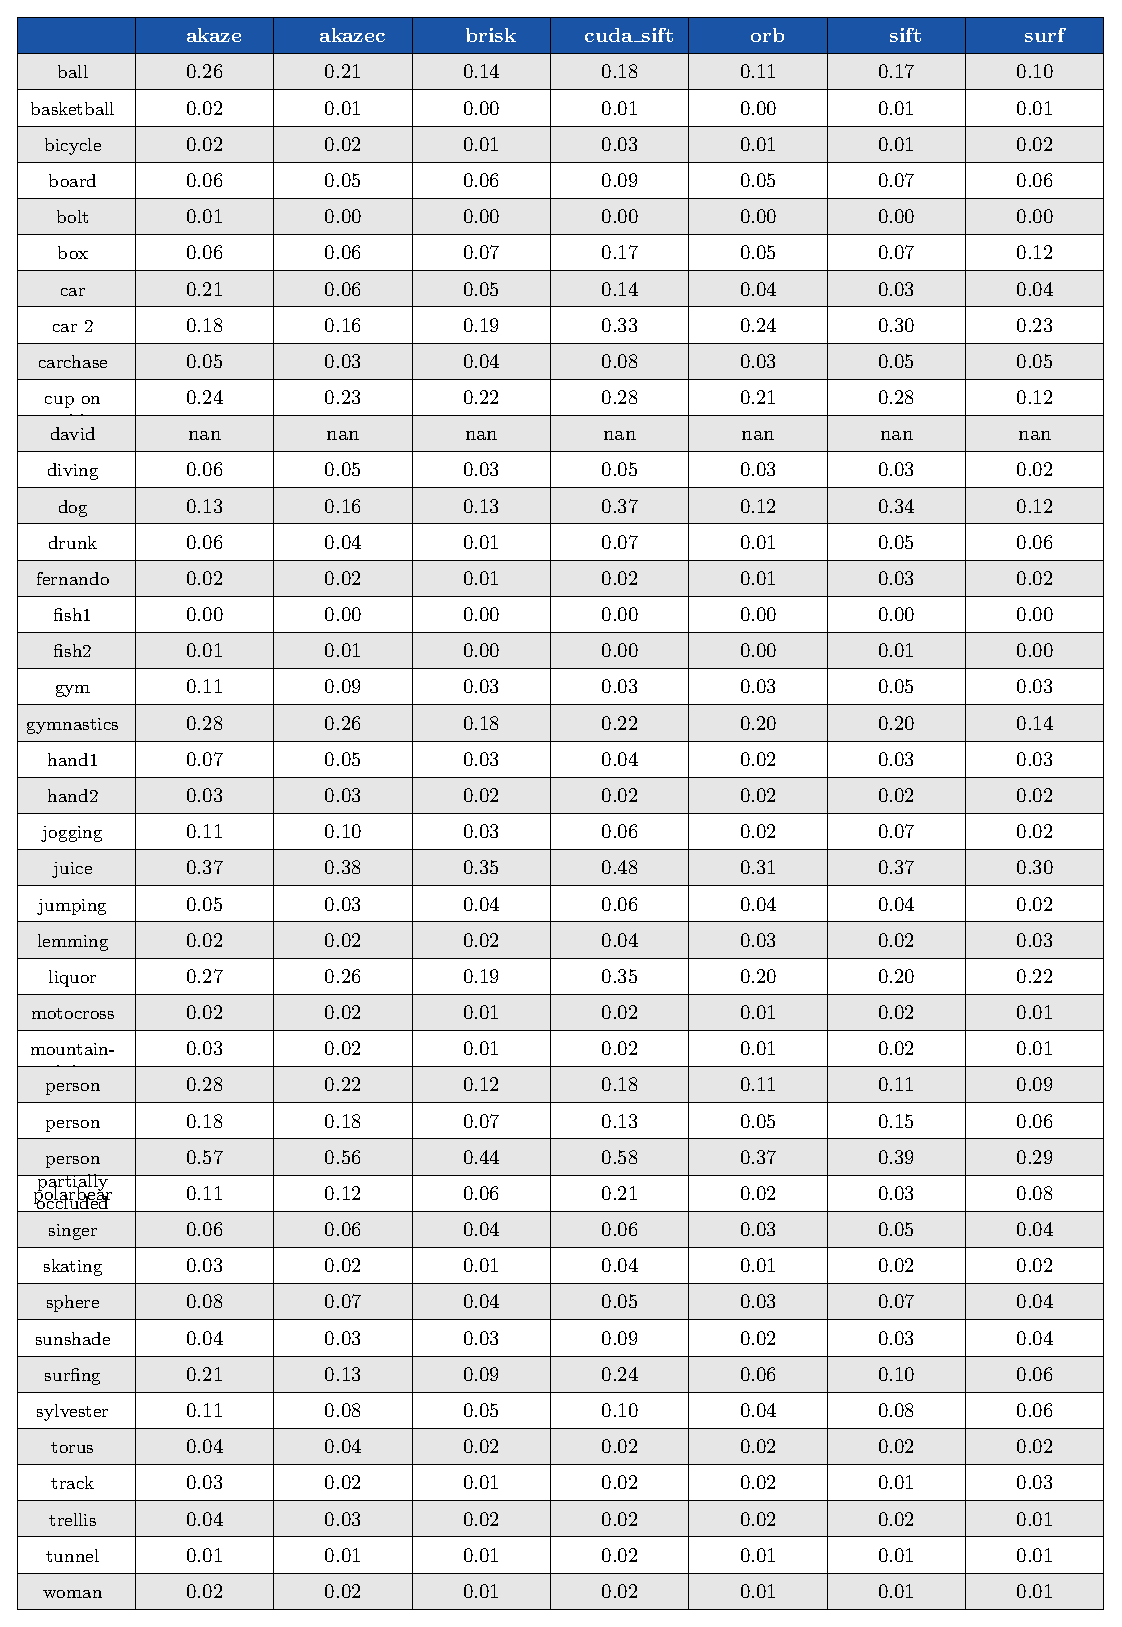
\includegraphics[width=0.98\linewidth]{tables/test.pdf}}
    \vspace{-2mm} 
	\caption{Overall results of the dataset for true positive matching. This is just a preview it won't be in he paper.}
	\label{fig:learnvsno}
\end{figure*}

